\documentclass[tikz,border=10pt]{standalone}
% Shared look for every TikZ diagram. Load with % Shared look for every TikZ diagram. Load with % Shared look for every TikZ diagram. Load with \input{../../tools/tikz-style.tex}
\usepackage[T1]{fontenc}
\usepackage{lmodern}
\renewcommand{\sfdefault}{lmr}  % diagrams use the same serif as the text
\usetikzlibrary{arrows.meta, positioning, shapes.geometric, calc, fit, backgrounds}
\definecolor{cblue}{HTML}{4C78A8}
\definecolor{corange}{HTML}{F58518}
\definecolor{cgreen}{HTML}{54A24B}
\definecolor{cred}{HTML}{E45756}
\definecolor{cpurple}{HTML}{B279A2}
\definecolor{cgrey}{HTML}{6B6B6B}
\tikzset{
  every picture/.style={font=\sffamily, line width=1.2pt},
  box/.style={draw=#1, fill=#1!12, rounded corners=4pt, align=center, inner sep=7pt, minimum height=1.1cm},
  box/.default=cgrey,
  arrow/.style={-{Stealth[length=3mm]}, draw=cgrey, line width=1.4pt},
  title/.style={font=\sffamily\bfseries\Large},
  note/.style={font=\sffamily\small, text=cgrey, align=center},
}
\AtBeginDocument{\hyphenpenalty=10000 \exhyphenpenalty=10000}

\usepackage[T1]{fontenc}
\usepackage{lmodern}
\renewcommand{\sfdefault}{lmr}  % diagrams use the same serif as the text
\usetikzlibrary{arrows.meta, positioning, shapes.geometric, calc, fit, backgrounds}
\definecolor{cblue}{HTML}{4C78A8}
\definecolor{corange}{HTML}{F58518}
\definecolor{cgreen}{HTML}{54A24B}
\definecolor{cred}{HTML}{E45756}
\definecolor{cpurple}{HTML}{B279A2}
\definecolor{cgrey}{HTML}{6B6B6B}
\tikzset{
  every picture/.style={font=\sffamily, line width=1.2pt},
  box/.style={draw=#1, fill=#1!12, rounded corners=4pt, align=center, inner sep=7pt, minimum height=1.1cm},
  box/.default=cgrey,
  arrow/.style={-{Stealth[length=3mm]}, draw=cgrey, line width=1.4pt},
  title/.style={font=\sffamily\bfseries\Large},
  note/.style={font=\sffamily\small, text=cgrey, align=center},
}
\AtBeginDocument{\hyphenpenalty=10000 \exhyphenpenalty=10000}

\usepackage[T1]{fontenc}
\usepackage{lmodern}
\renewcommand{\sfdefault}{lmr}  % diagrams use the same serif as the text
\usetikzlibrary{arrows.meta, positioning, shapes.geometric, calc, fit, backgrounds}
\definecolor{cblue}{HTML}{4C78A8}
\definecolor{corange}{HTML}{F58518}
\definecolor{cgreen}{HTML}{54A24B}
\definecolor{cred}{HTML}{E45756}
\definecolor{cpurple}{HTML}{B279A2}
\definecolor{cgrey}{HTML}{6B6B6B}
\tikzset{
  every picture/.style={font=\sffamily, line width=1.2pt},
  box/.style={draw=#1, fill=#1!12, rounded corners=4pt, align=center, inner sep=7pt, minimum height=1.1cm},
  box/.default=cgrey,
  arrow/.style={-{Stealth[length=3mm]}, draw=cgrey, line width=1.4pt},
  title/.style={font=\sffamily\bfseries\Large},
  note/.style={font=\sffamily\small, text=cgrey, align=center},
}
\AtBeginDocument{\hyphenpenalty=10000 \exhyphenpenalty=10000}

\begin{document}
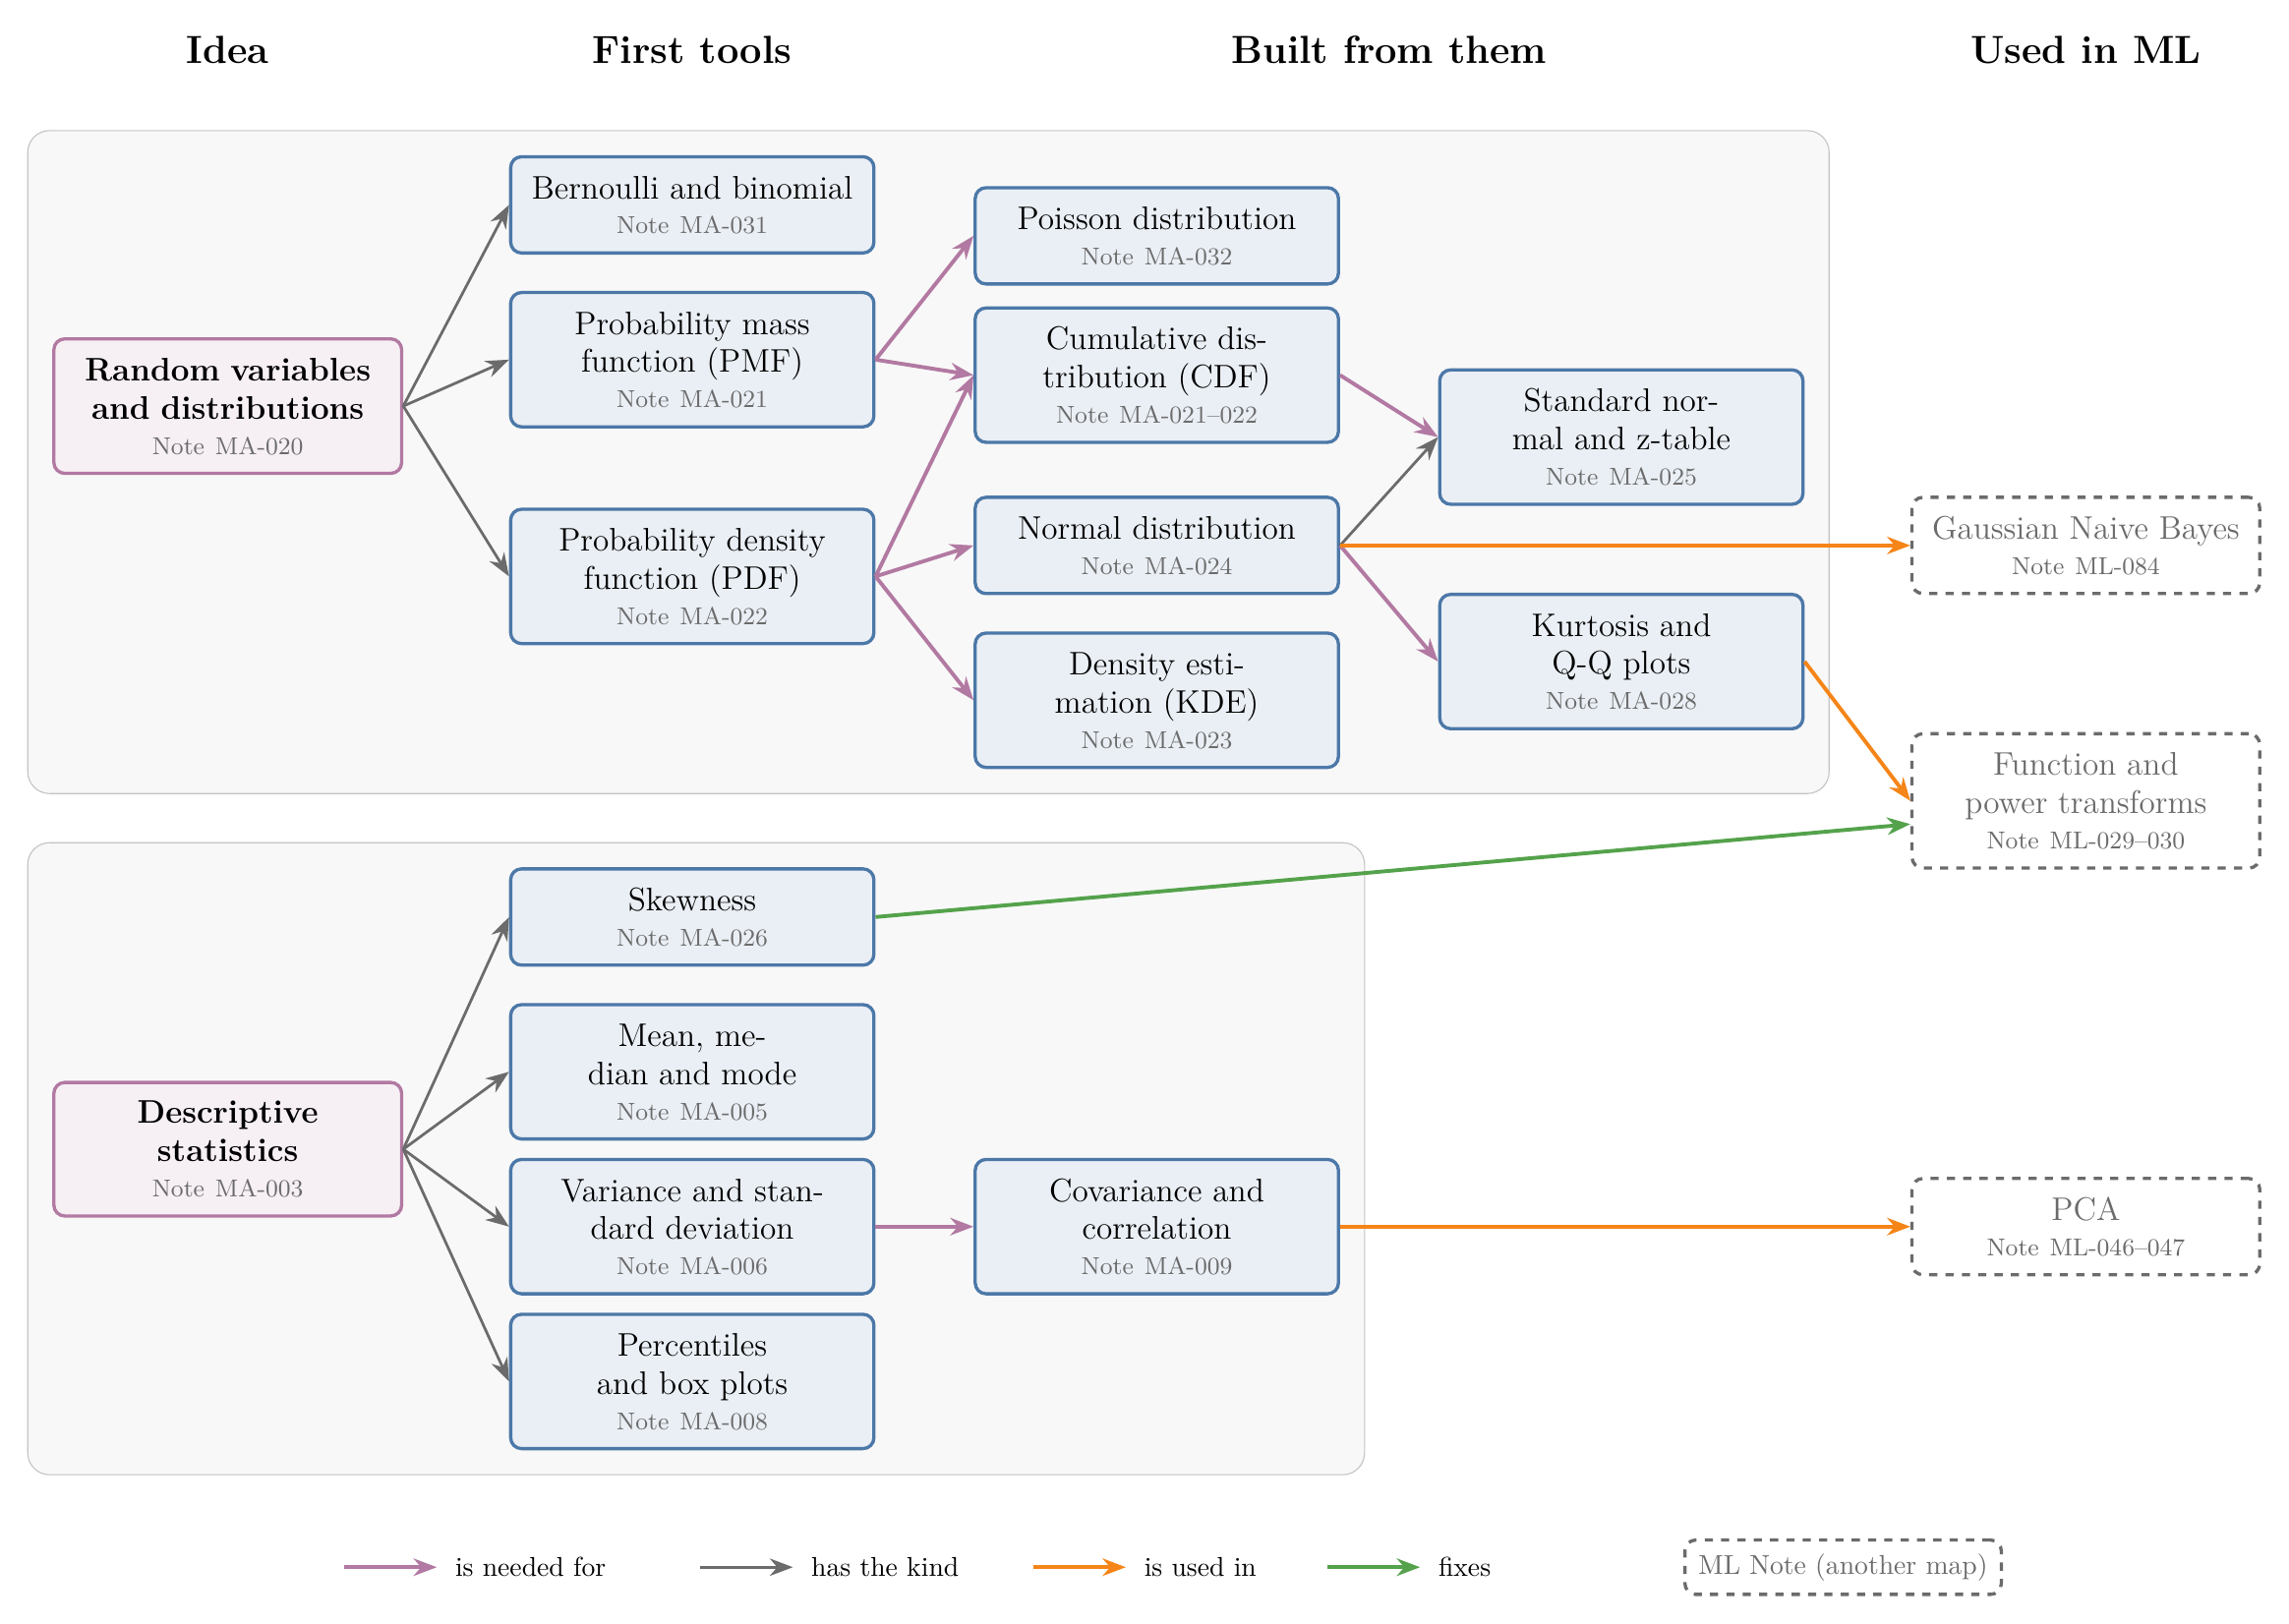
\begin{tikzpicture}[
    every node/.append style={font=\sffamily\large},
    idea/.style={box=cpurple, text width=4.0cm},
    con/.style={box=cblue, text width=4.2cm},
    prev/.style={draw=cgrey, dashed, rounded corners=4pt, align=center, inner sep=7pt, text=cgrey, text width=4.0cm, minimum height=1.1cm},
    group/.style={draw=cgrey!40, fill=cgrey!5, rounded corners=8pt, inner sep=9pt},
    needs/.style={arrow, draw=cpurple},
    kind/.style={arrow, draw=cgrey, line width=1pt},
    used/.style={arrow, draw=corange},
    fixes/.style={arrow, draw=cgreen},
  ]
  \newcommand{\nt}[1]{\\[-1pt]{\small\color{cgrey}Note #1}}
  \node[title] at (0,10.2)  {Idea};
  \node[title] at (6,10.2)  {First tools};
  \node[title] at (15,10.2) {Built from them};
  \node[title] at (24,10.2) {Used in ML};

  % ---- band 1: probability distributions
  \node[idea] (rv) at (0,5.6) {\textbf{Random variables and distributions}\nt{MA-020}};
  \node[con] (bin)  at (6,8.2) {Bernoulli and binomial\nt{MA-031}};
  \node[con] (pmf)  at (6,6.2) {Probability mass function (PMF)\nt{MA-021}};
  \node[con] (pdf)  at (6,3.4) {Probability density function (PDF)\nt{MA-022}};
  \node[con] (poi)  at (12,7.8) {Poisson distribution\nt{MA-032}};
  \node[con] (cdf)  at (12,6.0) {Cumulative distribution (CDF)\nt{MA-021--022}};
  \node[con] (nor)  at (12,3.8) {Normal distribution\nt{MA-024}};
  \node[con] (kde)  at (12,1.8) {Density estimation (KDE)\nt{MA-023}};
  \node[con] (std)  at (18,5.2) {Standard normal and z-table\nt{MA-025}};
  \node[con] (qq)   at (18,2.3) {Kurtosis and Q-Q plots\nt{MA-028}};

  % ---- band 2: descriptive statistics
  \node[idea] (desc) at (0,-4.0) {\textbf{Descriptive statistics}\nt{MA-003}};
  \node[con] (skew) at (6,-1.0) {Skewness\nt{MA-026}};
  \node[con] (ct)   at (6,-3.0) {Mean, median and mode\nt{MA-005}};
  \node[con] (var)  at (6,-5.0) {Variance and standard deviation\nt{MA-006}};
  \node[con] (box)  at (6,-7.0) {Percentiles and box plots\nt{MA-008}};
  \node[con] (cov)  at (12,-5.0) {Covariance and correlation\nt{MA-009}};

  % ---- ML uses
  \node[prev] (nb)  at (24,3.8)  {Gaussian Naive Bayes\nt{ML-084}};
  \node[prev] (pt)  at (24,0.5)  {Function and power transforms\nt{ML-029--030}};
  \node[prev] (pca) at (24,-5.0) {PCA\nt{ML-046--047}};

  \begin{scope}[on background layer]
    \node[group, fit=(rv) (bin) (poi) (kde) (std) (qq)] {};
    \node[group, fit=(desc) (skew) (box) (cov)] {};
  \end{scope}

  % distributions
  \draw[kind] (rv.east) -- (bin.west);
  \draw[kind] (rv.east) -- (pmf.west);
  \draw[kind] (rv.east) -- (pdf.west);
  \draw[needs] (pmf.east) -- (poi.west);
  \draw[needs] (pmf.east) -- (cdf.west);
  \draw[needs] (pdf.east) -- (cdf.west);
  \draw[needs] (pdf.east) -- (nor.west);
  \draw[needs] (pdf.east) -- (kde.west);
  \draw[kind]  (nor.east) -- (std.west);
  \draw[needs] (cdf.east) -- (std.west);
  \draw[needs] (nor.east) -- (qq.west);
  \draw[used]  (nor.east) -- (nb.west);
  \draw[used]  (qq.east) -- (pt.west);

  % descriptive
  \foreach \c in {skew, ct, var, box} \draw[kind] (desc.east) -- (\c.west);
  \draw[needs] (var.east) -- (cov.west);
  \draw[used]  (cov.east) -- (pca.west);
  \draw[fixes] (skew.east) -- ([yshift=-3mm]pt.west);

  % legend
  \begin{scope}[shift={(1.5,-9.4)}, every node/.style={font=\sffamily, anchor=west}]
    \draw[needs] (0,0) -- (1.2,0);     \node at (1.3,0) {is needed for};
    \draw[kind] (4.6,0) -- (5.8,0);    \node at (5.9,0) {has the kind};
    \draw[used] (8.9,0) -- (10.1,0);   \node at (10.2,0) {is used in};
    \draw[fixes] (12.7,0) -- (13.9,0); \node at (14.0,0) {fixes};
    \node[draw=cgrey, dashed, rounded corners=4pt, inner sep=5pt, text=cgrey, anchor=west] at (17.3,0) {ML Note (another map)};
  \end{scope}
\end{tikzpicture}
\end{document}
